\section{Auswertung}
\label{sec:Auswertung}
\subsection{Verifizierung der Linsengleichung}
Mit den Messdaten aus der Tabelle \ref{tab:ersterVersuchsteil} soll die Gleichung \ref{eq:linsengleichung} auf Gültigkeit überprüft werden und dementsprechend das Ergebnis mit dem vom Hersteller angegebenen Brennweite verglichen werden. Zudem sind die vom Hersteller Brennweiten wie folgt angegeben:
\begin{align*}
f_\text{Hersteller1} &= \SI{100 E-3}{\meter} \\
f_\text{Hersteller2} &= \SI{150 E-3}{\meter}. \\
\end{align*}

Der Mittelwert $\bar{f}$ aus $n$ Stichproben $f_{i}$ ergibt sich aus:
\begin{equation}
\bar{f}=\frac{1}{n}\sum \limits_{i=1}^n f_{i}
\label{eq:mittelwert}
\end{equation}
Die Standardabweichung errechnet sich nach:
\begin{equation}
\label{eq:standardab}
s_{i}= \sqrt{\frac{1}{n-1}\sum \limits_{i=1}^n(f_{i}-\bar{f})^2}
\end{equation}
mit zufälligen Fehlern behafteten Werten $f_{i}$ mit $i = 1,...,n$.\\
Der aus der Standardabweichung aus der Gleichung \ref{eq:standardab} resultierende Fehler des Mittelwertes ergibt sich nach:
\begin{equation}
\Delta\bar{f}=\frac{s_{i}}{\sqrt{n}} = \sqrt{\frac{\sum\limits_{i=1}^n(f_{i}-\bar{f})^2}{n(n-1)}}.
\label{eq:fehlermittelwert}
\end{equation}

\begin{table}[htpb]
	\centering
	\caption{Messwerte zur Bestimmung der Brennweite $f$.}
	\label{tab:ersterVersuchsteil}
	\begin{tabular}{c c c}
		\toprule
		$g / \si{\meter}$ & $b / \si{\meter}$ & $f_1 / \SI{E-3}{\meter}$ \\
		\midrule
		0,510 &	0,1210& 97,77 \\
		0,490&	0,1240& 98,95 \\
		0,470&	0,1250& 98,73 \\
		0,440&	0,1275& 98,85 \\
		0,400&	0,1320& 99,24 \\
		0,350&	0,1370& 98,45 \\
		0,300&	0,1460& 98,20 \\
		0,270&	0,1550& 98,47 \\
		0,220&	0,1780& 98,39 \\
		0,170&	0,2350& 98,64 \\	
		\midrule
		$g / \si{\meter}$ & $b / \si{\meter}$ & $f_2 / \SI{E-3}{\meter}$ \\
		\midrule
		0,260&	0,576& 179,13\\
		0,290&	0,583& 193,66\\
		0,330&	0,591& 211,75\\
		0,370&	0,608& 230,02\\
		0,400&	0,626& 244,05\\
		0,430&	0,646& 258,15\\
		0,460&	0,670& 283,01\\
		0,490&	0,695& 287,38\\
		0,520&	0,718& 301,58\\
		0,565&	0,763& 352,73\\
		\bottomrule
	\end{tabular}
\end{table}

Mit der Gleichung \ref{eq:mittelwert} und \ref{eq:fehlermittelwert} wird nun der Mittelwert sowie der Fehler des Mittelwerts der Brennweite $f_1$ und $f_2$ bestimmt und es ergeben sich die folgende Werte:
\begin{align*}
f_1 &= \SI{98,5 \pm 0,1 E-3}{\meter} \\
f_2 &= \SI{255,4 \pm 16,8 E-3}{\meter}.
\end{align*}

Die Genauigkeit der Messungen wird in Abbildung \ref{fig:messungen1} zusätzlich graphisch dargestellt. Hier werden die Gegenstandsweiten $g$ auf der x-Achse mit den dazugehörigen Bildweiten $b$ auf der y-Achse durch eine Gerade verbunden. Je genauer sich diese Geraden in einem Punkt, der dem Punkt $(f \mid f)$ entspricht, schneiden, desto genauer sind auch die Messungen. 

Eine lineare Ausgleichsgerade lässt sich berechnen wie:
\begin{equation}
\label{eq:ausgleichsgerade}
y = mx + b
\end{equation}
wobei $m$ die Steigung und $b$ der y-Achsenabschnitt sind. Über Formel \ref{eq:ausgleichsgerade} werden die Steigungen vom Python-Modul Scipy curve\_fit dargestellt.

\begin{figure}[h!]
	\centering
	\includegraphics[width=0.7\linewidth]{../../Messungen1}
	\caption{Messungenauigkeit für die Brennweite $f= \SI{100}{\milli\meter}$}
	\label{fig:messungen1}
\end{figure}

Aus der Abbildung \ref{fig:messungen1} lässt sich den Schnittpunkt $S$ ablesen und es folgt:
\begin{equation*}
S = (0,098 \mid 0,1).
\end{equation*}

Als nächstes wird für die andere bekannte Brennweite $f = \SI{150}{\milli\meter}$ das gleiche Verfahren wiederholt. Die Genauigkeit der Messungen wird in Abbildung \ref{fig:messungen2} zusätzlich graphisch dargestellt. Über Formel \ref{eq:ausgleichsgerade} werden die Steigungen vom Python-Modul Scipy curve\_fit dargestellt.

Aus der Abbildung \ref{fig:messungen2} lässt sich den Schnittpunkt $S$ ablesen und es folgt:
\begin{equation*}
S = (-0,2 \mid 0,9).
\end{equation*}

\begin{figure}[h!]
	\centering
	\includegraphics[width=0.7\linewidth]{../../Messungen2}
	\caption{Messungenauigkeit für die Brennweite $f= \SI{150}{\milli\meter}$.}
	\label{fig:messungen2}
\end{figure}

\subsection{Bestimmung der Brennweite nach der Methode von Bessel}
Für die nächste Linse wird die Methode von Bessel verwendet, um die Brennweite bestimmen zu können. Bei der Messung mit weißem Licht werden für $10$ verschiedene Abstände $e$, jeweils $g_1$, $g_2$ und $b_1$, $b_2$ bestimmt. Die Messdaten und die ausgerechneten Brennweiten nach der Gleichung \ref{eq:bessel} befinden sich in der Tabelle \ref{tab:zweiterVersuchsteil}.

\begin{table}[htpb]
	\centering
	\caption{Messwerte zur Bestimmung der Brennweite $f$ nach der Methode von Bessel.}
	\label{tab:zweiterVersuchsteil}
	\begin{tabular}{c c c c c c c c c }
		\toprule
		$g_1 / \si{\meter}$ & $b_1 / \si{\meter}$ & $b_2 /\si{\meter}$ & $g_2/ \si{\meter}$ & $e / \si{\meter}$ & $d_2 / \si{\meter}$ & $d_1 / \si{\meter}$ & $d / \si{\meter}$& $f / \SI{E-3}{\meter}$  \\
		\midrule
	    0,1135 &0,9065 & 0,1120 &0,9080 & 1,02 & 0,796 & 0,793& 0,794 $\pm$ 0,0015 & 0,104 $\pm$ 0,006 \\
	    0,1145 &0,8665 & 0,1115 &0,8685 & 0,98 & 0,751 & 0,751& 0,754 $\pm$ 0,003 & 0,096 $\pm$ 0,001 \\
	    0,1150 &0,8250 & 0,1120 &0,8280 & 0,94 & 0,710 & 0,710& 0,713 $\pm$ 0,003 & 0,088 $\pm$ 0,001 \\
	    0,1155 &0,7845 & 0,1125 &0,7875 & 0,90 & 0,669 & 0,669& 0,672 $\pm$ 0,003 & 0,081 $\pm$ 0,001 \\
 	    0,1160 &0,7440 & 0,1140 &0,7460 & 0,86 & 0,628 & 0,628& 0,630 $\pm$ 0,002 & 0,073 $\pm$ 0,005 \\
	    0,1170 &0,7130 & 0,1140 &0,7160 & 0,83 & 0,596 & 0,596& 0,599 $\pm$ 0,003 & 0,068 $\pm$ 0,007 \\
	    0,1190 &0,6410 & 0,1160 &0,6440 & 0,76 & 0,522 & 0,522& 0,525 $\pm$ 0,003 & 0,057 $\pm$ 0,005 \\
	    0,1225 &0,5575 & 0,1200 &0,5600 & 0,68 & 0,435 & 0,435& 0,4375 $\pm$ 0,0025 & 0,046 $\pm$ 0,003 \\
	    0,1250 &0,4950 & 0,1440 &0,4760 & 0,62 & 0,370 & 0,370& 0,351 $\pm$ 0,019 & 0,040 $\pm$ 0,002 \\
	    0,1300 &0,4200 & 0,1320 &0,4180 & 0,55 & 0,290 & 0,290& 0,288 $\pm$ 0,002 & 0,030 $\pm$ 0,001 \\
		\bottomrule
	\end{tabular}
\end{table}

Um $d$ bestimmen zu können, müssen zuerst die Abstände $d_1$ und $d_2$ nach der Gleichung \ref{eq:mittelwert} gemittelt werden und entsprechend der Fehler des Mittelwerts auch nach der Gleichung \ref{eq:fehlermittelwert} ausgerechnet werden. Hierbei muss die Gaußsche Fehlerfortpflanzung eingebaut werden, da es sich um fehlerbehaftete Größen handelt und es ergibt sich:
\begin{equation}
\label{eq:fehlergauß}
\Delta f = \sqrt{\left(\frac{\partial f}{\partial d}\right)^2 \cdot \Delta d^2} = \sqrt{\left(\frac{-d}{2e}\right)^2 \cdot \Delta d^2}.
\end{equation}

Mit der Gleichung \ref{eq:mittelwert} und \ref{eq:fehlermittelwert} wird nun der Mittelwert sowie der Fehler des Mittelwerts der Brennweite $f$ bestimmt und es ergibt sich der folgende Wert:
\begin{equation*}
f = \SI{68,5 \pm 7,8 E-3}{\meter},
\end{equation*}
wobei die Brennweite vom Hersteller wieder $f_\text{Hersteller1} =  \SI{100}{\milli\meter}$ ist. 

Um die chromatische Abberation mit derselben Methode zu untersuchen, werden jeweils ein roter und blauer Filter benötigt. Die Messdaten mit den entsprechenden Farbfilter und die ausgerechneten Brennweiten nach \ref{eq:bessel} befinden sich in den Tabelle \ref{tab:zweiteraVersuchsteil} und \ref{tab:zweiterbVersuchsteil}. Hier wird $d$ für die beiden Filter analog wie im vorherigen Verfahren berechnet. Nach der Gleichung \ref{eq:fehlergauß} werden die Fehler der Brennweiten ausgerechnet.

\begin{table}[htpb]
	\centering
	\caption{Messwerte zur Bestimmung der Brennweite $f$ nach der Methode von Bessel für den roten Filter.}
	\label{tab:zweiteraVersuchsteil}
	\begin{tabular}{c c c c c c c c c}
		\toprule
		$g_1 / \si{\meter}$ & $b_1 / \si{\meter}$ & $b_2 /\si{\meter}$ & $g_2/ \si{\meter}$ & $e / \si{\meter}$ & $d_2 / \si{\meter}$ & $d_1 / \si{\meter}$ & $d / \si{\meter}$& $f_\text{rot} / \SI{E-3}{\meter}$  \\
		\midrule
  		0,1220 & 0,711 &0,116 & 0,717 & 0,833 & 0,601 & 0,589 & 0,595 $\pm$ 0,006 & 0,071 $\pm$ 0,001\\
  		0,1230 & 0,627 &0,118 & 0,632 & 0,750 & 0,514 & 0,504 & 0,509 $\pm$ 0,005 & 0,056 $\pm$ 0,009\\
  		0,1300 & 0,490 &0,125 & 0,495 & 0,620 & 0,370 & 0,360 & 0,365 $\pm$ 0,005 & 0,038 $\pm$ 0,005\\
  		0,1470 & 0,323 &0,139 & 0,331 & 0,470 & 0,192 & 0,176 & 0,184 $\pm$ 0,008 & 0,021 $\pm$ 0,003\\
  		0,1855 & 0,2145&0,117 & 0,223 & 0,400 & 0,046 & 0,029 & 0,037 $\pm$ 0,008 & 0,015 $\pm$ 0,006 \\
		\bottomrule
	\end{tabular}
\end{table}

\begin{table}[htpb]
	\centering
	\caption{Messwerte zur Bestimmung der Brennweite $f$ nach der Methode von Bessel für den blauen Filter.}
	\label{tab:zweiterbVersuchsteil}
	\begin{tabular}{c c c c c c c c c}
		\toprule
		$g_1 / \si{\meter}$ & $b_1 / \si{\meter}$ & $b_2 /\si{\meter}$ & $g_2/ \si{\meter}$ & $e / \si{\meter}$ & $d_2 / \si{\meter}$ & $d_1 / \si{\meter}$ & $d / \si{\meter}$& $f_\text{blau} / \SI{E-3}{\meter}$  \\
		\midrule
         0,118 & 0,802 & 0,114 & 0,806 & 0,92 & 0,692 & 0,684 & 0,688 $\pm$ 0,005 & 0,085 $\pm$ 0,001 \\
         0,120 & 0,700 & 0,115 & 0,705 & 0,82 & 0,590 & 0,580 & 0,585 $\pm$ 0,007 & 0,067 $\pm$ 0,001 \\
         0,123 & 0,597 & 0,118 & 0,602 & 0,72 & 0,484 & 0,474 & 0,479 $\pm$ 0,007 & 0,052 $\pm$ 0,008 \\
         0,129 & 0,491 & 0,124 & 0,496 & 0,62 & 0,372 & 0,362 & 0,367 $\pm$ 0,007 & 0,038 $\pm$ 0,005 \\
         0,136 & 0,384 & 0,131 & 0,389 & 0,52 & 0,258 & 0,248 & 0,253 $\pm$ 0,007 & 0,023 $\pm$ 0,003 \\
		\bottomrule
	\end{tabular}
\end{table}

Mit der Gleichung \ref{eq:mittelwert} und \ref{eq:fehlermittelwert} wird nun der Mittelwert sowie der Fehler des Mittelwerts der Brennweite $f_\text{rot}$ und $f_\text{blau}$ bestimmt und es ergeben sich die folgende Werte:
\begin{align*}
f_\text{rot} &= \SI{40,8 \pm 10,3 E-3}{\meter} \\
f_\text{blau} &= \SI{54,2 \pm 23,3 E-3}{\meter}.
\end{align*}

\subsection{Bestimmung der Brennweite nach der Methode von Abbe}
Um die Brennweite eines Linsensystems nach der Methode von Abbe zu bestimmen, werden für $10$ Gegenstandsweiten $g'$ die Bildweite $b'$ gemessen, damit die Hauptebenen $h$ und $h'$ und Brennweite $f$ eines Linsensystems zu bestimmen. Zudem werden die Gleichungen nach \ref{eq:abbemethode} benötigt. Die dazu gehörigen Messwerte befinden sich in der Tabelle \ref{tab:dritterVersuchsteil}. Dabei ergibt sich der Abbildungsmaßstab über Gleichung \ref{eq:abbildungsgesetz}.

\begin{table}[htpb]
	\centering
	\caption{Messwerte zur Bestimmung der Brennweite $f$ nach der Methode von Abbe.}
	\label{tab:dritterVersuchsteil}
	\begin{tabular}{c c c c c c c c}
		\toprule
		$\text{Referenzpunkt A} / \si{\meter}$ &$G / \si{\meter}$ & $B / \si{\meter}$ & $g' / \si{\meter}$ & $b' / \si{\meter}$ & $V$ & $1+V$ & $1 + \frac{1}{V}$ \\
		\midrule
         1,08 &0,031 & 0,067 & 0,18 & 0,685 & 2,16 & 3,16 & 1,46 \\
         1,06 &0,031 & 0,054 & 0,20 & 0,619 & 1,74 & 2,74 & 1,57 \\
         1,03 &0,031 & 0,040 & 0,23 & 0,511 & 1,29 & 2,29 & 1,77 \\
         1,00 &0,031 & 0,033 & 0,26 & 0,468 & 1,06 & 2,06 & 1,93 \\ 
         0,97 &0,031 & 0,026 & 0,29 & 0,460 & 0,83 & 1,83 & 2,19 \\
         0,94 &0,031 & 0,023 & 0,32 & 0,438 & 0,74 & 1,74 & 2,34 \\
         0,91 &0,031 & 0,021 & 0,35 & 0,422 & 0,67 & 1,67 & 2,47 \\
         0,88 &0,031 & 0,019 & 0,38 & 0,415 & 0,61 & 1,61 & 2,63 \\
         0,85 &0,031 & 0,016 & 0,41 & 0,402 & 0,51 & 1,51 & 2,93 \\
         0,82 &0,031 & 0,014 & 0,44 & 0,394 & 0,45 & 1,45 & 3,21 \\
		\bottomrule
	\end{tabular}
\end{table}

In Abbildung \ref{fig:abbe1} wird die Gegenstandweite $g'$ gegen $1+\frac{1}{V}$ aufgetragen und in Abbildung \ref{fig:abbe2} wird die Bildweite $b'$ gegen $1+V$ aufgetragen. Über Formel \ref{eq:ausgleichsgerade} wird die Steigung und der Fehler der Ausgleichsgerade vom Python-Modul Scipy curve\_fit berechnet.
Es ergaben sich für die Ausgleichsgerade $m$ als Steigung und $b$ als y-Achsenabschnitt die folgenden Werte für die erste Ausgleichsgerade:
\begin{align*}
m &= \SI{153 \pm 5 e-3}{\meter} \\
b &= \SI{40,3 \pm 11,7 e-3}{\meter}
\end{align*}
und für die zweite:
\begin{align*}
m &= \SI{171,5 \pm 7,3 e-3}{\meter} \\
b &= \SI{136,5 \pm 15,1 e-3}{\meter}.
\end{align*}

\begin{figure}[h!]
	\centering
	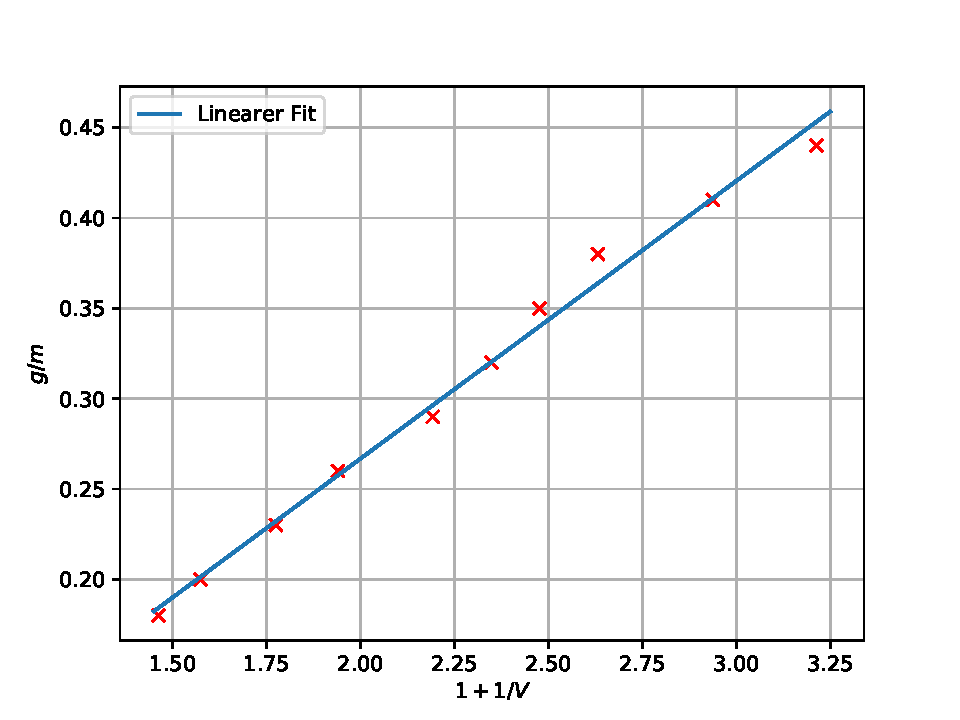
\includegraphics[width=0.7\linewidth]{../../Abbe1}
	\caption{Regression mit Gegenstandsweite.}
	\label{fig:abbe1}
\end{figure}

\begin{figure}
	\centering
	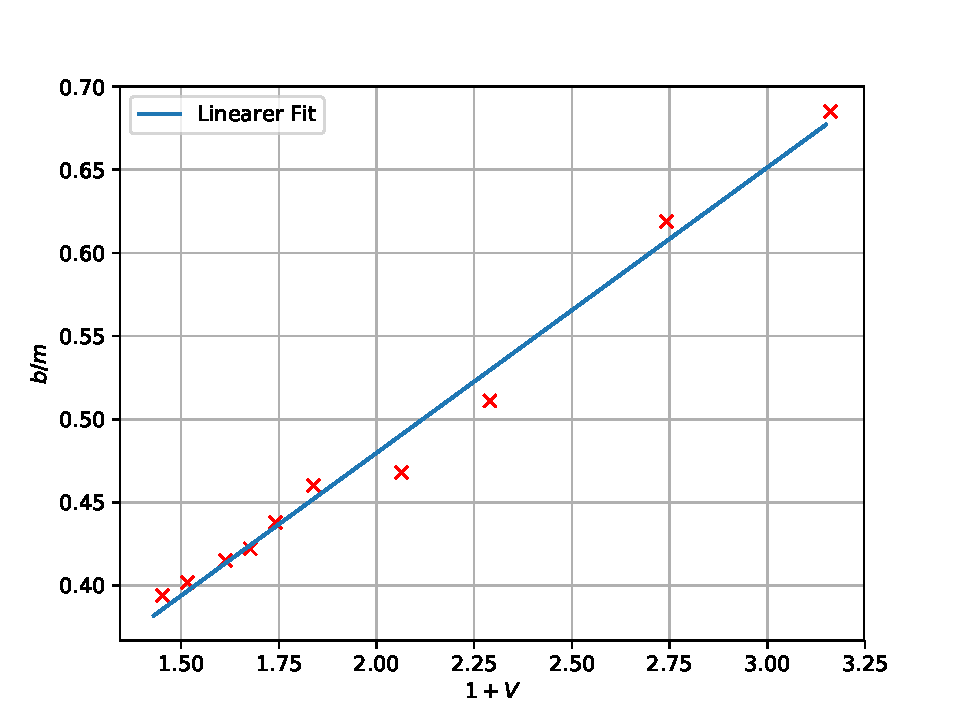
\includegraphics[width=0.7\linewidth]{../../Abbe2}
	\caption{Regression mit Bildweite.}
	\label{fig:abbe2}
\end{figure}

Die Brennweite $f$ und die Abstände $h$ und $h'$ ergeben sich durch einen Vergleich der Gleichungen \ref{eq:abbemethode}:
\begin{align*}
f_g &= \SI{153 \pm 5 e-3}{\meter} \\
f_b &= \SI{171,5 \pm 7,3 e-3}{\meter} \\
h &= \SI{40,3 \pm 11,7 e-3}{\meter} \\
h' &= \SI{136,5 \pm 15,1 e-3}{\meter}.
\end{align*}

Die Lage der Hauptachsen lauten dann $H = A + h$ und $H' = A + h'$.